\chapter{Implementacja}
\label{cha:implementacja}

Ze względu na to, że omawiana aplikacja składa się z autonomicznych elementów, znaczna część implementacji poszczególnych serwisów mogła odbywać się niezależnie od innych. Tworzone funkcjonalności testowane były przy pomocy narzędzia Postman, za pomocą którego można wysyłać dowolnie skonfigurowane zapytania HTTP na konkretne adresy URI. Kolejne, gotowe usługi były następnie integrowane w systemie.

%---------------------------------------------------------------------------

\section{Metodyka pracy}
Projekt powstawał iteracyjnie. To znaczy, że podczas pracy zaczynano od małych celów i po ich realizacji - stawiano większe, aż do osiągnięcia zamierzonego efektu. Udoskonalano obecny wówczas stan i przechodzono do kolejnego, bardziej zaawansowanego kroku. W ten sposób,możliwe było dokładne kontrolowanie rozwoju systemu, jego testowanie i w razie problemów - szybka analiza, znalezienie i wyeliminowanie przyczyny. 

\subsection{Version Control System}
\textbf{VCS} - postęp prac śledzony był za pomocą systemu kontroli wersji.
Pozwala on dokumentować każdą, kolejną zmianę, która ma miejsce w odniesieniu do kodu. Dzięki temu wygodniejsze są wszelkie zmiany związane z nowymi elementami w kodzie, ponieważ\\w każdym momencie, możliwy jest powrót do dowolnego, poprzedniego stanu implementowanych funkcjonalności.~\cite{vcs}
W projekcie korzystano z hostingu na platformie GitHub.

\subsection{Organizacja zadań}
\textbf{Kanban} to metodologia, która może być użyta jako narzędzie do zarządzania projektem podczas produkcji oprogramowania. Oryginalnie została wymyślona w celu optymalizacji produkcji w Japońskiej firmie Toyota.

\newpage
Jej wykorzystanie w procesie rozwijania systemów informatycznych znacząco wzrasta ze względu na jej przewagę nad tradycyjnymi metodami. Objawia się ona w elastyczności, wydajności i zwiększonej produktywności. Sama nazwa oznacza w wolnym tłumaczeniu ``spis widoczny``.~\cite{kanban}

Najbardziej charakterystycznym elementem jest utworzenie swojego rodzaju torów, oznaczających poszczególne etapy w których znajdują się obecnie zadania. W momencie zmiany stanu, dany element jest przemieszczany do następnej w kolejności kolumny, co oznacza, że zadanie jest coraz bliżej ukończenia.\newline
Korzystając z faktu, że w serwisie Github możliwe jest utworzenie takiej kanbanowej tablicy, zdecydowano się na użycie właśnie tej implementacji narzędzia. Poniżej zaprezentowano stan części planszy podczas rozwoju projektu.
\begin{figure}[H]
	\centering
	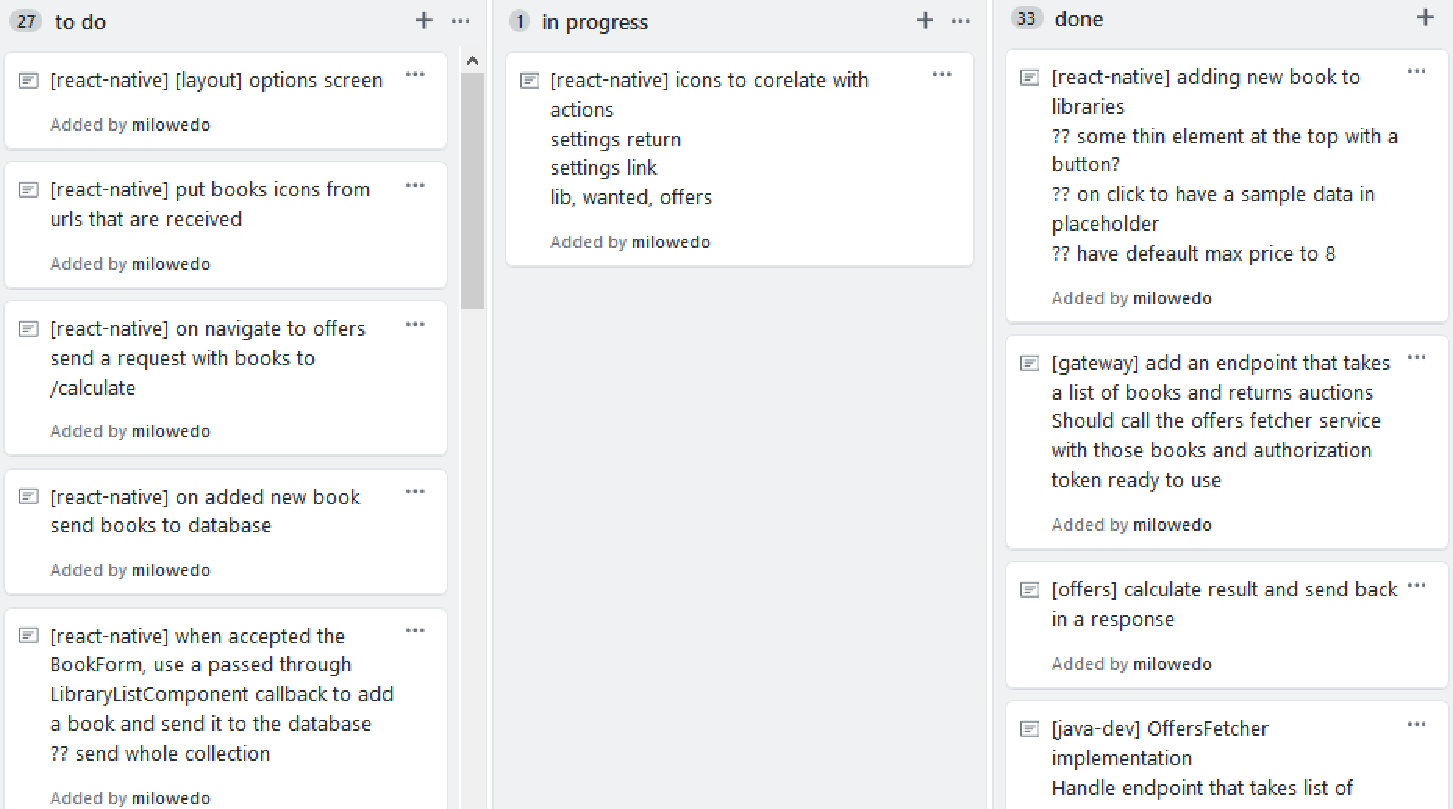
\includegraphics[width=\linewidth]{kanban.pdf}
	\caption{\centering Kanbanowa tablica podzielona na 3 sektory}
	\caption*{\centering Źródło: {Opracowanie własne - zrzut ekranu z projektu na platformie Github.com}}
\end{figure}

%---------------------------------------------------------------------------
\newpage
\section{Wybór technologii}
Językami programowania, które mają największy udział w projekcie są Javascript (2.2, 2.3, 2.7) oraz Java (2.4).\newline
Za persystencję odpowiada chmurowa wersja bazy danych NoSQL (2.6.2) - MongoDB Cloud.

\subsection{Express}
\textbf{Auth Service} (2.2) oraz \textbf{Gateway} (2.3) to serwisy o podobnym stosie technologicznym. Obydwa powstały z pomocą Express js API - javascriptowego frameworku wspierającego implementację serwera obsługującego tworzenie i wystawianie REST API.
\begin{figure}[H]
	\centering
	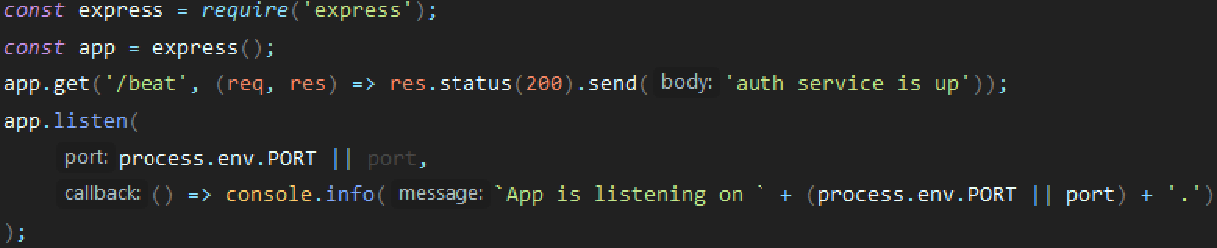
\includegraphics[width=\linewidth]{express_simple.pdf}
	\caption{\centering Elementarny kod odpowiedzialny za wystawienie prostego API za pomocą Express js}
	\caption*{\centering Źródło: {Opracowanie własne}}
\end{figure}
Jak przedstawiono powyżej, aby stworzyć nasłuchujący na jednym punkcie końcowym serwer, wystarczy parę linijek kodu. Naturalnie, potrzeby występujących w pracy serwisów są większe i potrzebują bardziej rozbudowanego podejścia niż przedstawiono na załączonej grafice.

\subsection{React Native}
\textbf{Aplikacja mobilna} jest napisana przy wykorzystaniu platformy Expo, która jest zestawem narzędzi ułatwiającym prace w stworzonym przez Facebook, Inc. frameworku mobilnym - React Native. Został on wybrany, ponieważ jest sprawdzony(popularne aplikacje, które używają go w swojej implementacji to między innymi Facebook, Instagram, Skype). Jest ciągle udoskonalany i prawdopodobnie nie przestanie być popularny w najbliższym czasie. Posiada on także pokaźną społeczność programistów, co zawsze jest nieocenionym atutem podczas korzystania z dowolnej technologii.

\newpage
Ciekawym rozwiązaniem zaprezentowanym przez twórców są tak zwane `Hooki`, które pozwalają używać stanu w wykorzystanych w omawianej aplikacji komponentach funkcyjnych - lżejszych niż komponenty klasowe.\newline
Jednym z przykładów zastosowania ich w aplikacji jest pobieranie książek(za pomocą funkcji fetchMyBooks()) z bazy danych - wywołanie to potrzebne jest jedynie raz, podczas pierwszego ładowania ekranu MyLibraryScreen. Nie jest pożądanym wysyłać zapytania za każdym razem, kiedy użytkownik powróci do tego samego ekranu. Tracone są wtedy bez potrzeby zasoby urządzenia - dane są już i tak obecne w pamięci podręcznej, więc nic nowego takie zachowanie nie przyniesie.
\begin{figure}[H]
	\centering
	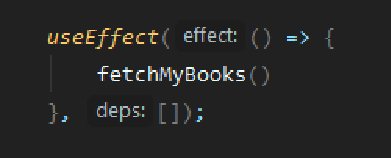
\includegraphics{hook.pdf}
	\caption{\centering Zastosowanie hooka ``useEffect``}
	\caption*{\centering Źródło: {Opracowanie własne}}
\end{figure}
Na powyższej grafice widać, że Hook \textbf{useEffect} przyjmuje dwa argumenty, pierwszy to funkcja, która ma się wykonać przy inicjalizacji komponentu oraz za każdym razem kiedy element tablicy z drugiego argumentu ulegnie zmianie.

%---------------------------------------------------------------------------

\section{Wielowątkowe tworzenie ofert}
Mając na uwadze fakt, że użytkownicy aplikacji mobilnej byliby najprawdopodobniej dużo mniej zadowoleni, jeżeli musieliby długo czekać na rezultat analizy ofert książek, zdecydowano się zwrócić szczególną uwagę na optymalizację tego czasochłonnego procesu.
Serwis OffersFetcher (2.4) jest aplikacją napisaną w frameworku Spring Boot. Przyjmując zapytanie w postaci listy książek, zwraca przygotowane oferty bazując na aktualnych\\w czasie rzeczywistym aukcjach na platformie Allegro.pl\newline
Dla każdej pozycji tworzone jest zadanie, które składa się następnie z podzadań. Wszystkie podzadania wykonywane są asynchronicznie i podzielone są w ten sposób, aby maksymalnie ograniczyć czas, w którym zasoby maszyny nie są wykorzystywane z powodu chociażby oczekiwania na odpowiedź z zewnętrznego serwisu Allegro.
\begin{figure}[H]
	\centering
	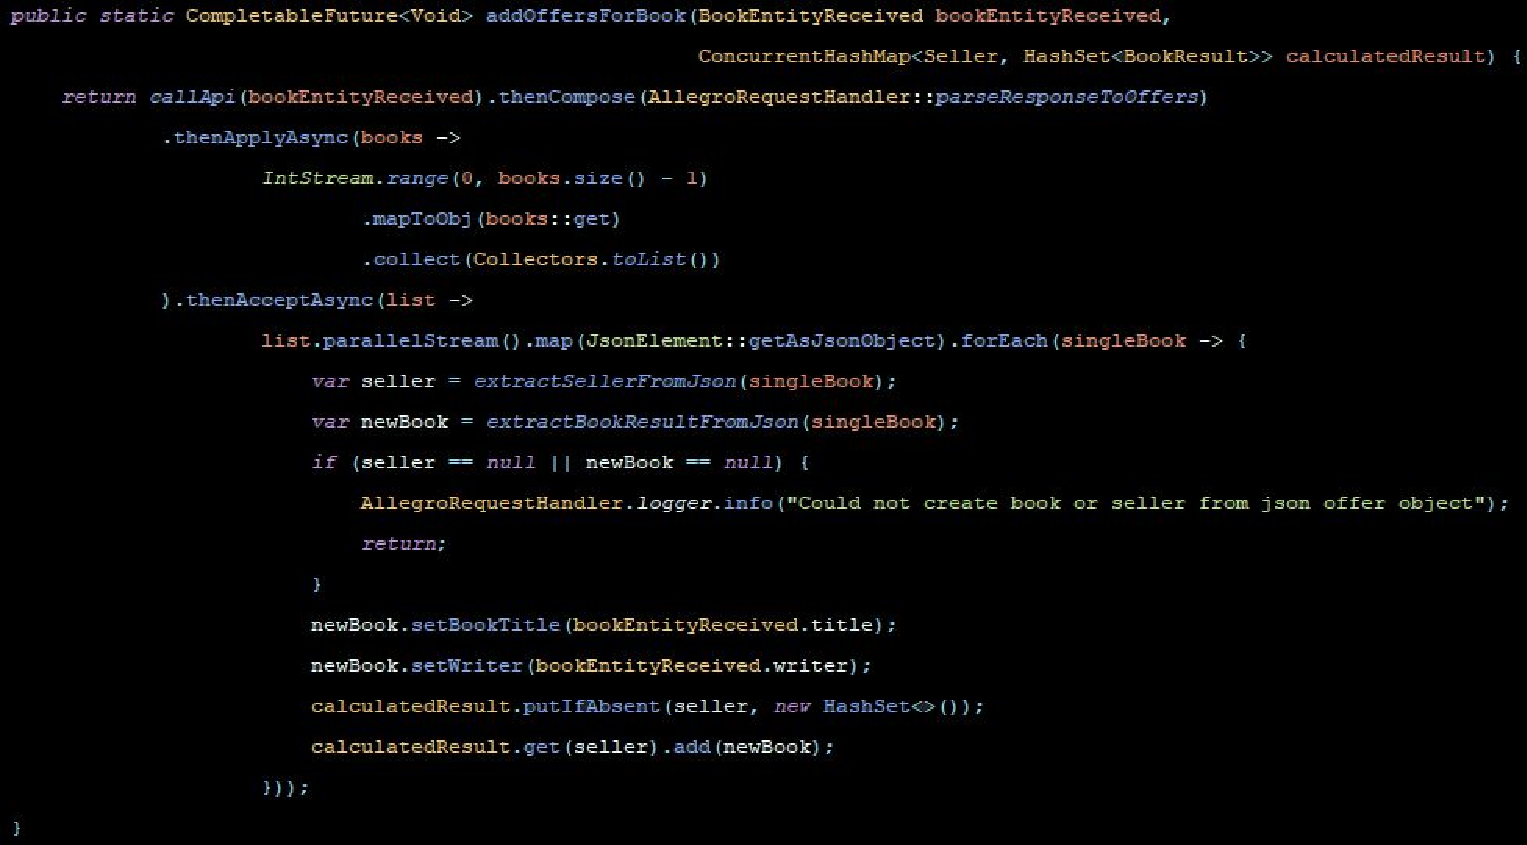
\includegraphics[width=\linewidth]{tasks.pdf}
	\caption{\centering Metoda wołana dla każdej książki z zapytania w serwisie OffersFetcher (2.4)}
	\caption*{\centering Źródło: {Opracowanie własne}}
\end{figure}
Na powyższej grafice widać główną logikę, odpowiedzialną za pobranie i zapisanie książek w wynikowej kolekcji. Jako argumenty, metoda przyjmuje obiekt reprezentujący pojedynczą książkę otrzymaną w zapytaniu oraz mapę zawierającą sprzedawców i do tej pory dopasowane do nich poszukiwane pozycje, znajdujące się w ich ofercie.
W pierwszej kolejności wywoływana jest metoda, która wysyła zapytanie typu GET do Allegro REST API. Następnie, jeżeli podzadanie zostanie wykonane i otrzymana zostanie odpowiedź, tekst jest przetwarzany kolejno do postaci tablicy i następnie do listy obiektów typu JSON.
Na koniec, po pozytywnym wyniku wykonania poprzednich kroków, strumieniowo analizowane są wszystkie pozycje i przydzielane są odpowiednim sprzedawcom.

%---------------------------------------------------------------------------

\section{Autoryzacja użytkownika w Allegro API}

Do integracji serwisu z aplikacją potrzebne jest pozyskanie tokenu dostępowego. Allegro udostępnia tzw. \textit{ścieżkę device flow}, dzięki której cały proces odbywa się bez konieczności uwzględniania go w interfejsie graficznym. Poniżej zaprezentowany jest diagram prezentujący tę funkcjonalność.

\begin{figure}[H]
	\centering
	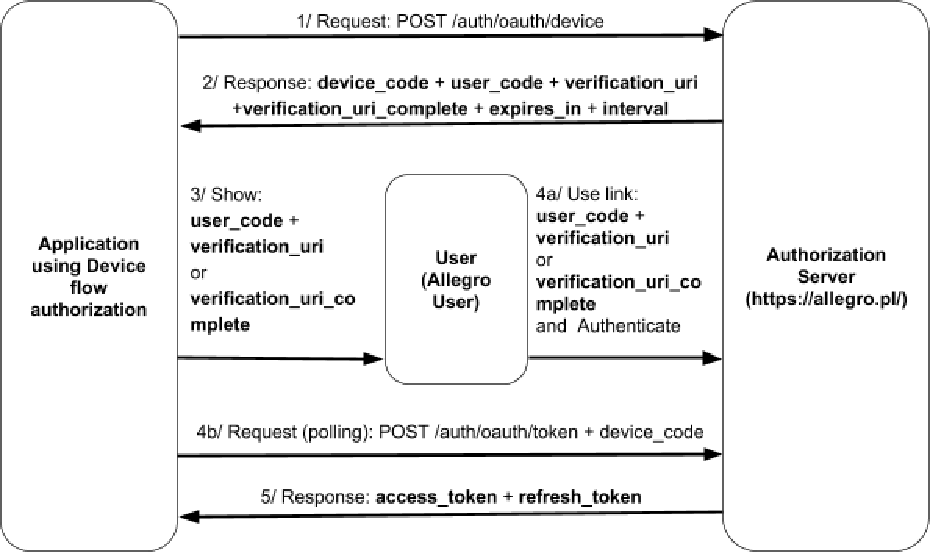
\includegraphics[width=\linewidth]{device_flow.pdf}
	\caption{\centering Autoryzacja użytkownika typu Device flow}
	\caption*{\centering Źródło: {https://developer.allegro.pl/}}
\end{figure}

Podejście w poniższej pracy zakłada zarejestrowanie jednego, wspólnego dla całego systemu, konta funkcjonalnego za pomocą którego każde zapytanie będzie autentykowane. Stwarza to niestety jedno ograniczenie. Mianowicie, ze względu na obowiązujący główny limit nakładany na Client ID  - po przekroczeniu liczby 9000 zapytań na minutę, aplikacja zwróci kod błędu 429 i zostanie zablokowana na kolejne 60 sekund.\newline
W fazie inicjalizacyjnej autoryzacji uzyskane zostaną dwa unikalne tokeny: 
\begin{itemize}
	\item dostępowy - ważny przez 12h
	\item odświeżający - ważny 6 miesięcy
\end{itemize}
Zostaną one zachowane w pamięci, a każde kolejne zapytanie, w przypadku wygaśnięcia tokenu dostępowego, spowoduje jego odnowienie.
\begin{figure}[H]
	\centering
	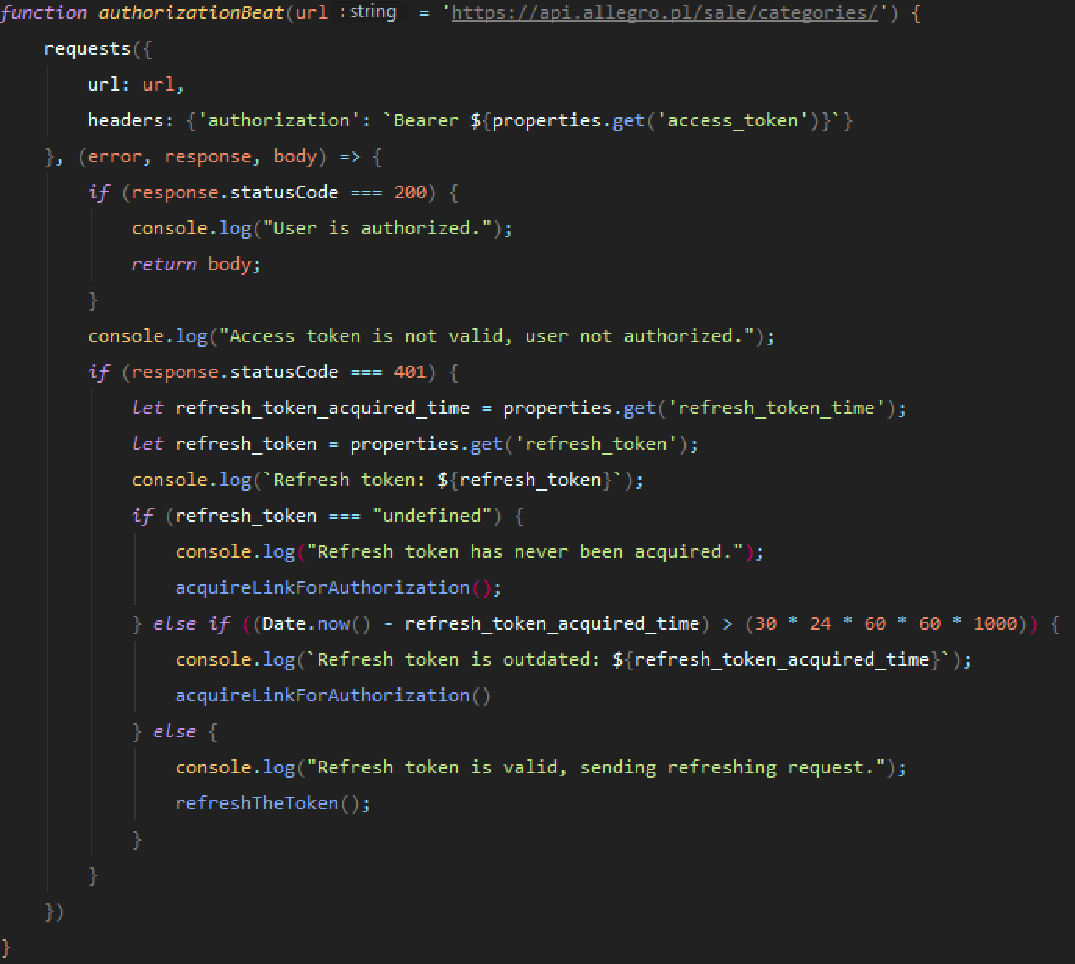
\includegraphics[width=\linewidth]{authorization.pdf}
	\caption{\centering Kod odpowiedzialny za utrzymywanie ważnego tokena}
	\caption*{\centering Źródło: {Opracowanie własne}}
\end{figure}
Powyższy kod prezentuje przebieg akcji, które mają miejsce za każdym razem, kiedy otrzymywane jest zapytanie do OffersService (2.4). Na początku sprawdzane jest, czy token jest zwyczajnie aktualny, następnie, w przypadku, gdy nie jest, pobierany jest token odświeżający. W zależności od tego, czy jest on ważny, wygasły, czy może w ogóle nigdy nie został uzyskany, odpowiednia logika zostaje uruchomiona.

%---------------------------------------------------------------------------
\newpage
\section{MongoDB Cloud}
Modele przechowujące dane są zdefiniowane w klasach Book.js oraz User.js serwisów Gateway (2.3) i Auth Service (2.2). Połączenie do bazy danych jest obsłużone przy pomocy biblioteki \textit{mongoose}.\newline
W celu uzyskania dostępu potrzebny jest jedynie tak zwany \textit{connection string}, który uzyskany został poprzez zalogowanie się na stronie webowej serwisu hostującego cloud.mongodb.com i nawigację do zakładki Connect.
\begin{figure}[H]
	\centering
	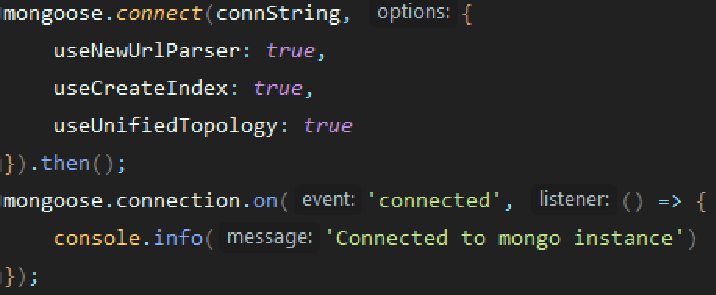
\includegraphics[width=\linewidth]{mongo.pdf}
	\caption{\centering Połączenie do bazy danych MongoDB}
	\caption*{\centering Źródło: {Opracowanie własne}}
\end{figure}
W załączonej grafice widać rozpoczęcie połączenia z bazą danych. Ważnym elementem jest opcja \textbf{useCreateIndex}, dzięki której znajdujące się w serwisach Auth Service i Gateway, modele, otrzymają indeksy pod którymi znaleźć będzie można zapisane dokumenty. 

%---------------------------------------------------------------------------

\section{Wdrożenie}

Korzystanie ze stworzonych serwisów jest umożliwione poprzez wdrożenie ich na platformie chmurowej Heroku.
W ten sposób każda usługa posiada własne URI, na które wysyłane są zapytania w zależności od potrzeb.
Poszczególne aplikacje można by również uruchomić na pojedynczym komputerze, jednakże wymagałoby to sporej ilości zasobów, stąd zdecydowano się na rozwiązanie hostingowe.

\newpage
Minimalne środowisko jakie jest wymagane aby uruchomić system to:
\begin{itemize}
	\item Node v10.13.0
	\item Java v11
	\item Maven v3.5
	\item Gradle v6.0
	\item Expo v3.11.1
\end{itemize}

Wdrożenie wymagało dodatkowo stworzenia aplikacji w sensie logicznym według platformy Heroku. Odbyło się to za pomocą linii komend Heroku CLI oraz poprzez wskazanie adresu URI do stosownych repozytoriów Github, gdzie przetrzymywany jest kod.
W ten sposób w webowym interfejsie pod adresem dashboard.heroku.com znalazły się odnośniki reprezentujące trzy usługi : OffersFetcher (2.4), Auth Service (2.2) oraz Gateway (2.3).\newline Każda z nich ma zdefiniowaną odpowiednią konfigurację, dzięki której aplikacje mogą zostać uruchomione.
\begin{itemize}
	\item {OffersFetcher (2.4) uruchamiany jest na platformie poleceniem \textit{web java -jar build/libs/*.jar}}
	\item {AuthService (2.2) oraz Gateway (2.3) - komendą \textit{npm start}}
\end{itemize}

Serwis reprezentujący bazę danych nie potrzebował bezpośredniego wdrożenia w postaci umieszczenia w konkretnym miejscu, napisanego wcześniej kodu. Cały proces uruchomienia bazy danych został wykonany za pomocą webowego interfejsu.

Aby uruchomić lokalnie aplikację mobilną należy w folderze ją zawierającym wykonać polecenie \textit{expo r}. Następnie w zainstalowanej na urządzeniu mobilnym aplikacji ``Expo`` w zakładce Projects pojawi się instancja aplikacji.

%---------------------------------------------------------------------------